\chapter{Implementation}
\label{ch:implementation}

[Brief introduction of the chapter]

~

Being a blockchain project, the goal is to not use the so called Web2 technologies, this means the traditional approaches of having a backend running on a server and similar services, but rather to use only Web3 technologies for us to understand exactly the limitations there are by adopting solely the blockchain ecosystem. Ideally, of course, in the future this project benefits greatly by merging these two approaches.

We'll be doing the smart contracts in Solidity, because it's the most popular language for Ethereum smart contracts, and makes it easy to deploy to any EVM compatible blockchain. This language can be similar to other languages like C++, but it has some unique features that make it very powerful for smart contracts.

Modifiers are a good example of this as they allow you to add custom logic to functions, can be used to prevent reentrancy attacks, which are a common security issue in smart contracts, and restrict the access to certain functions. We can define, for example, a call to register an event to be restricted to only organizers or a call to validate tickets to be limited to only validators. This is possible because there are a few keywords like \textit{msg.sender} that tell us which user address called the function and \textit{msg.value} that tells us how much value (ether) was sent with the transaction. This value is essentially the amount of money the user sends in a transaction, necessary for example to buy the tickets. We'll check if the value matches the total price and reverts otherwise.

\section{Main Smart Contract}
\label{sec:main_smart_contract}

So smart contracts are similar to C++ mainly because it lies on a class-like structure with variables to store data and methods, where the main difference is that a class is called a contract and you can extend others to integrate their functionalities. That's essentially what's gonna happen with each event, extending the ERC721 standard, making it a collection of NFTs, where each NFT is a ticket.

Since this is the behavior we want (each event being a NFT collection), we will have to deploy (instantiate, in C++) a new contract for each event, so we need a main contract to keep track of these events.

With this in mind, like we see in the Figure \ref{fig:system_uml}, the main contract will track the organizers and the events associated with the system, with the method to register a new event with the necessary data, restricted to only organizers (to avoid unauthorized people to interact), along with the necessary setters and getters and other system configurations.

\begin{figure}[H]
    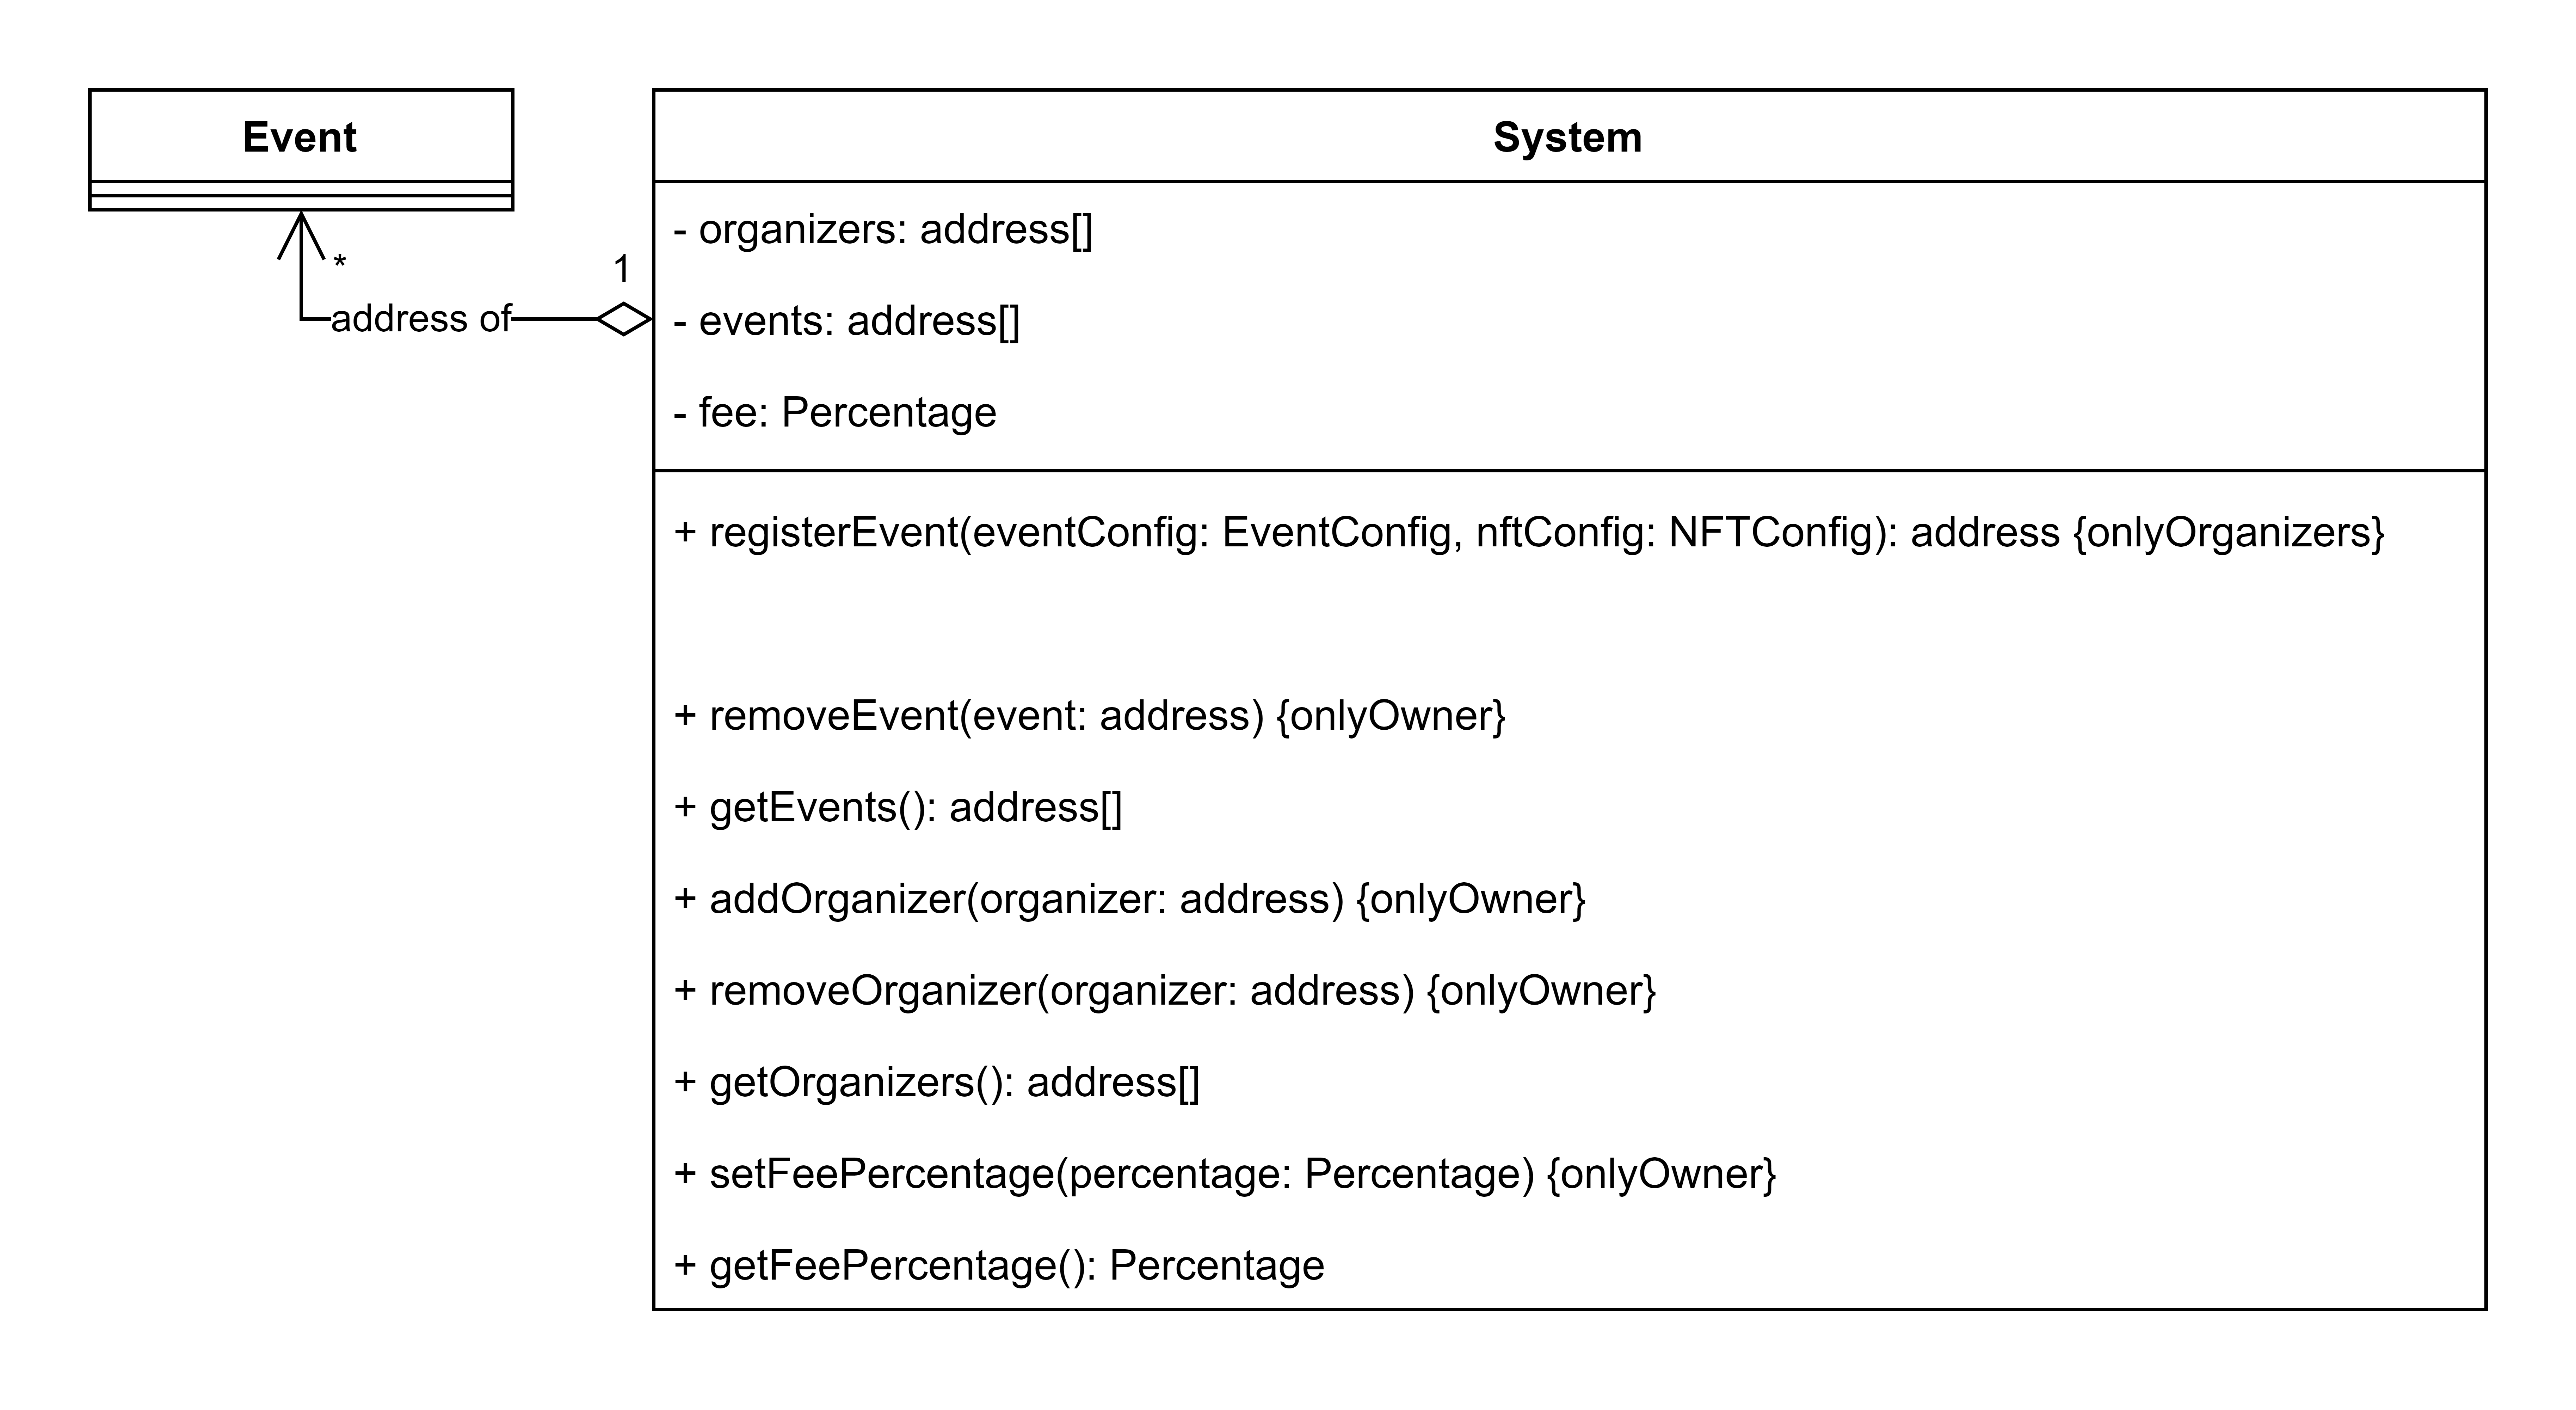
\includegraphics[width=\textwidth]{System UML.png}
    \centering
    \caption{Main smart contract UML}
    \label{fig:system_uml}
\end{figure}

Another unique feature of Solidity is the \textit{address} type, which is basically a string strict to the Ethereum address format. That's how we'll be storing the addresses of the organizers and the events that are deployed with the \textit{registerEvent} method. On the blockchain the only difference between a user and a contract is that a contract has code associated with it, so it can execute functions and store data, while a user can only send transactions.

With this structure, since we have this main contract where all the events of the system are stored, we can simply make a call to get them all, showcasing them in the app's home page for users to search.

\section{Event Smart Contract}
\label{sec:event_smart_contract}

For the event contract, we'll be extending the ERC721 standard and adding the necessary methods to interact with the tickets, like buying, selling, and validating them. The reason to extend this standard and not implement the logic manually is because it makes it compatible with the most common marketplaces for NFTs, which allows for users to do what they desire with them after the event. It also has the necessary methods to manage the tickets, like transferring them between users, and the necessary operations to track these operations.

\subsection{ERC721 Structure}
\label{subsec:erc721_structure}

The standard was obtained through the \href{https://docs.openzeppelin.com/contracts/api/token/erc721#ERC721}{OpenZeppelin} library, which is a collection of secure and community-vetted smart contracts that are used by many projects in the Ethereum ecosystem. This library is a great resource for developers to build secure and reliable smart contracts. The Figure \ref{fig:erc721_uml} shows us the most important variables and methods of the standard.

\begin{figure}[H]
    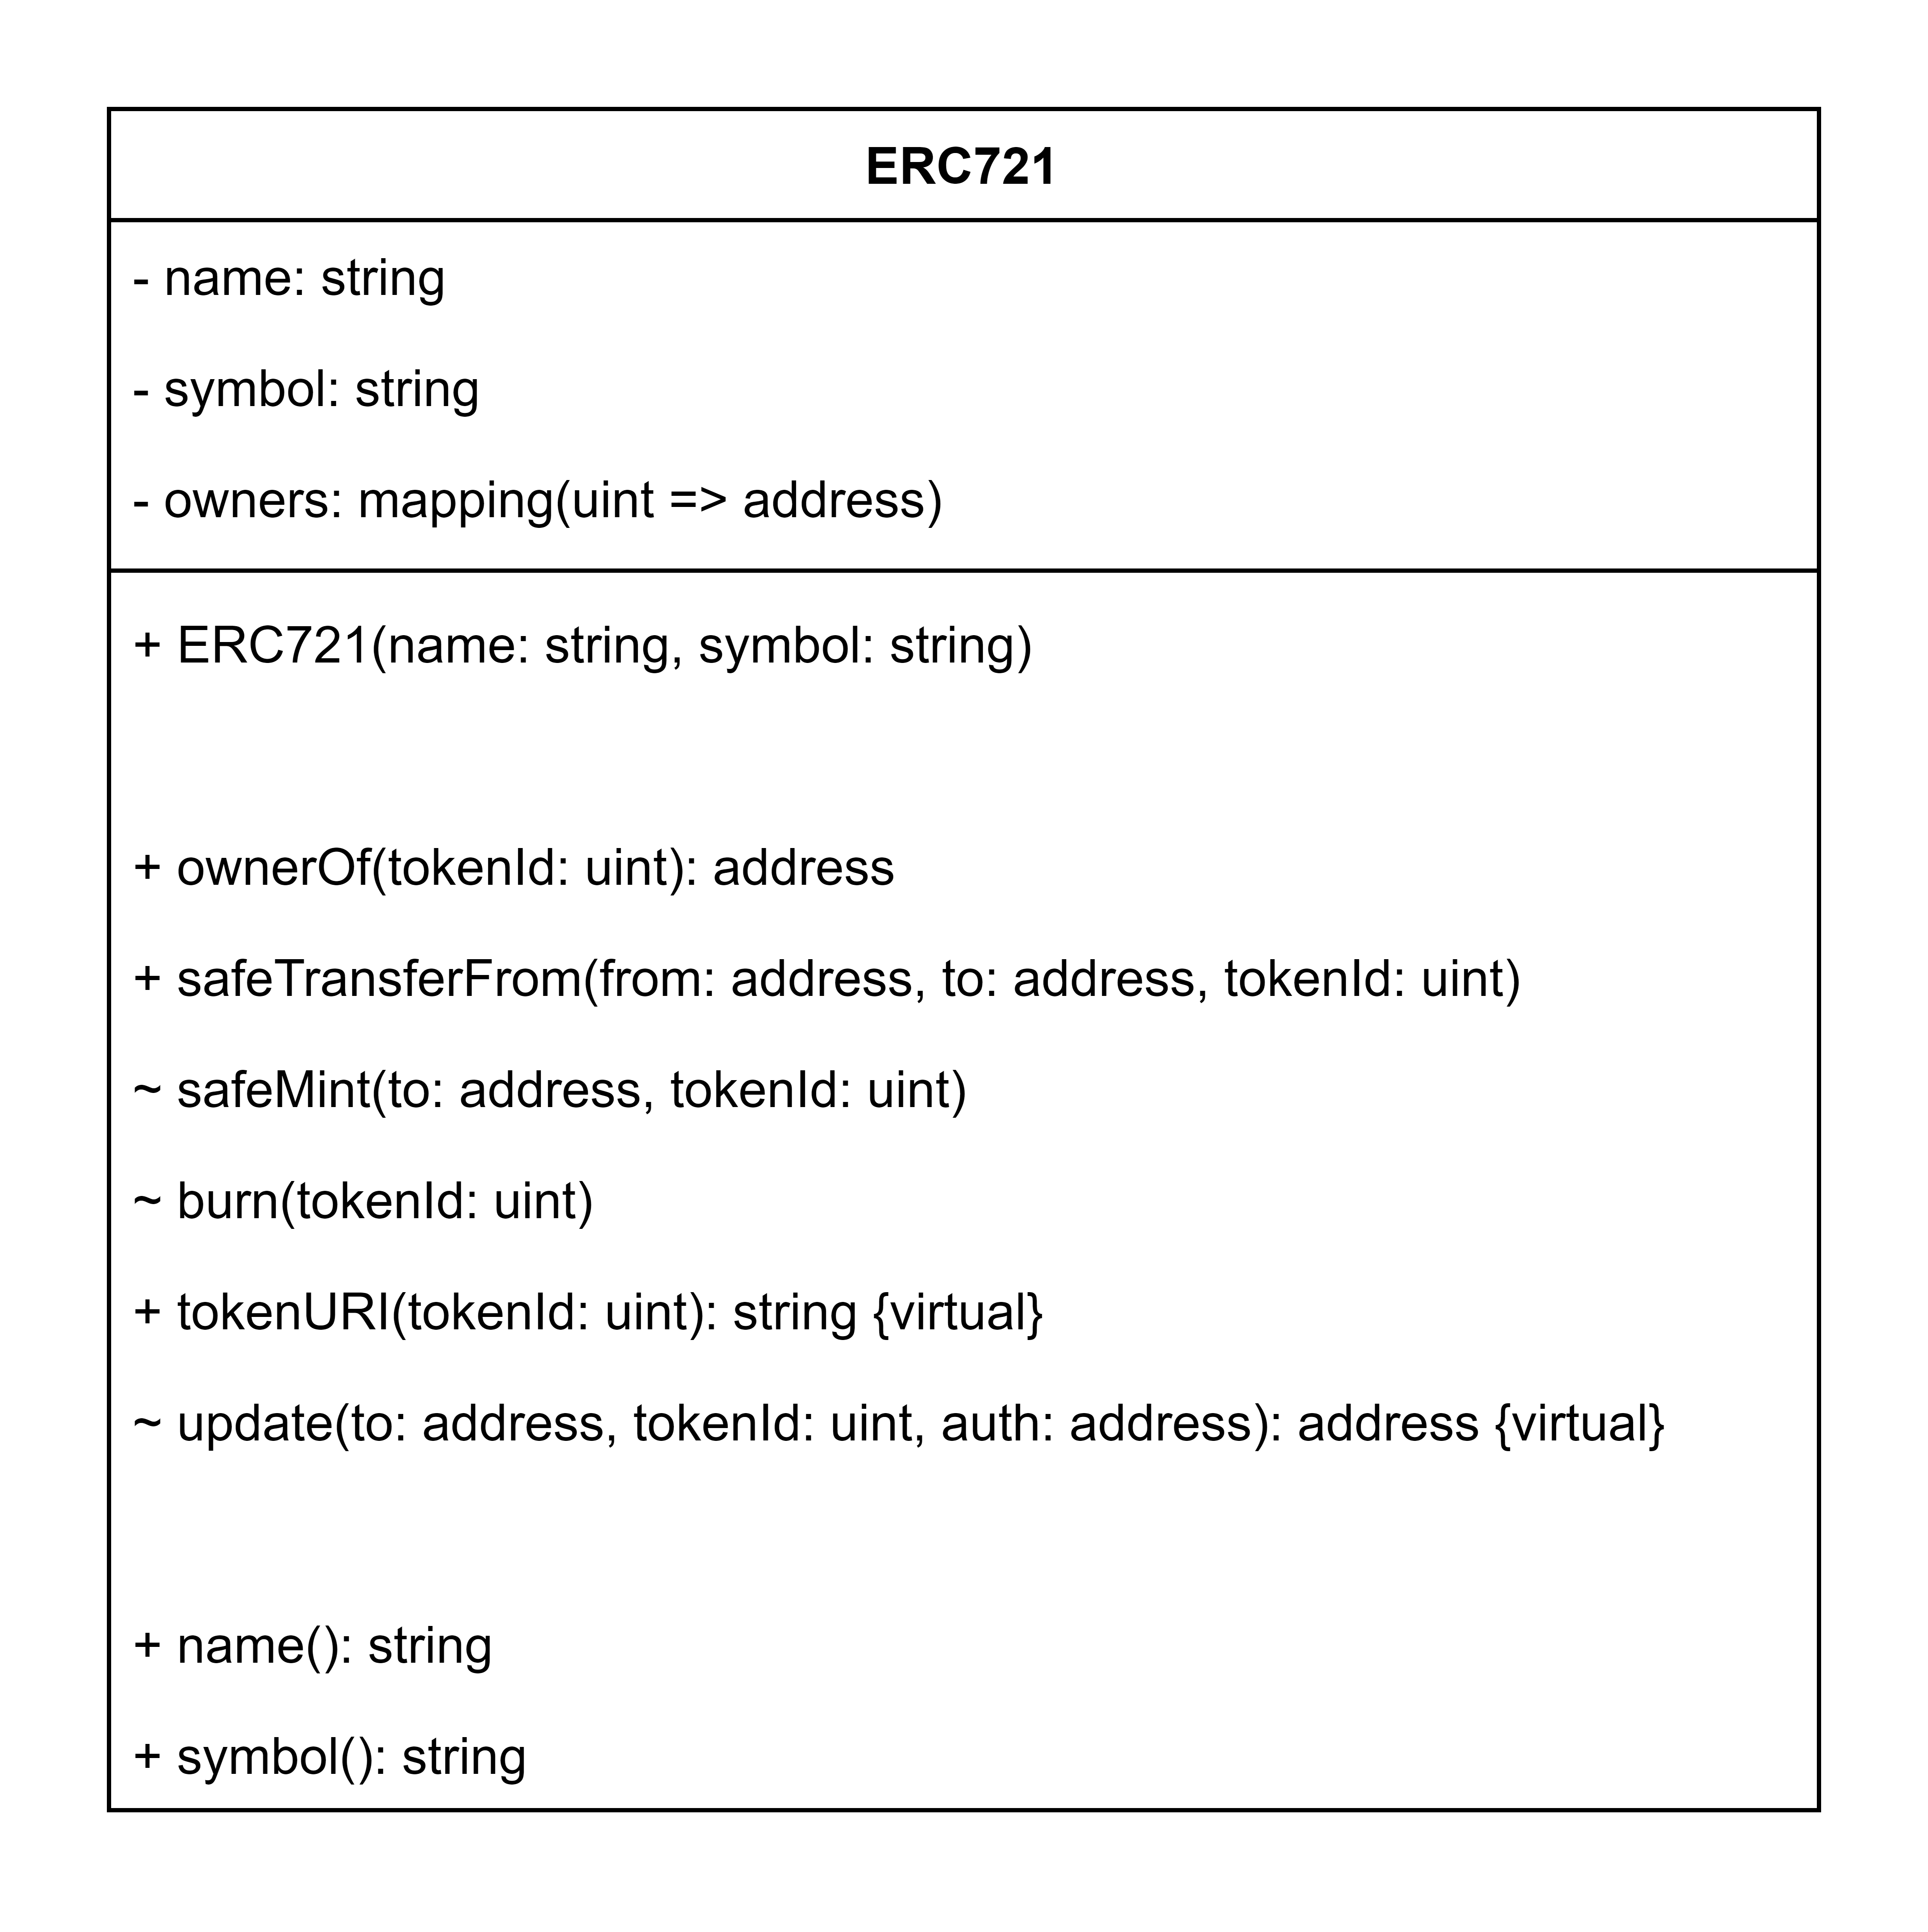
\includegraphics[width=\textwidth*2/3]{ERC721 UML.png}
    \centering
    \caption{ERC721 UML}
    \label{fig:erc721_uml}
\end{figure}

Analyzing its source code [ref] we can understand that the NFTs are simply a mapping of the token ID to the owner address, so when you execute a transaction to get a token (this process is called minting), the token ID is then associated to your address. Then for each token it's possible set a URI, which is a link to the NFTs metadata, usually being a JSON file with the necessary information about the token, like the name, description, and image.

This link could point to anything, for example a google drive file, but the common thing is to store the metadata on the IPFS, which is a decentralized storage system, so the metadata is not stored on the blockchain itself (onchain), which would be very expensive, but rather on a decentralized storage system (offchain), which is much cheaper.

The function \textit{tokenURI} is the one that is called by default in the marketplaces to get the metadata, being one of the main reasons to extend the ERC721 standard, because it enforces the implementation of this method. In the Figure \ref{fig:erc721_uml} we see it with the \textit{virtual} keyword, meaning this can be overridden by the contracts that extend it, to manipulate the way to store the metadata. We'll be mentioning this again in the Section [packages], about how the packages logic will be implemented.

    [structs]

    [mention storage]
    [event smart contract]
- [creation of events]
-- [ipfs (pinata)]
- [structs]
- [event lifecycle]
- [restrictions on ticket operations]

[ticket validation]
[todo mention network fees and network choice]

[user app]
[validator app]

\section{Project Features}
